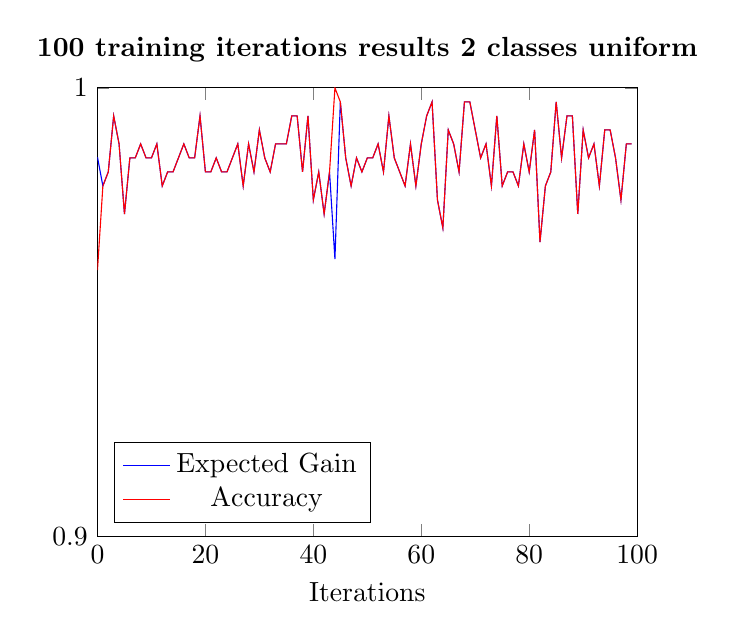
\begin{tikzpicture}
  \begin{axis}[
      title=\textbf{100 training iterations results 2 classes uniform},
      xlabel={Iterations},
      xmin=0, xmax=100,
      ymin=0.9, ymax=1,
      xtick={0,20,40,60,80,100},
      ytick={0.9,1.0},
      legend pos=south west,
      ymajorgrids=true,
      grid style=dashed,
  ]
  
  \addplot[color=blue, mark=dot]
    coordinates {
      (0,0.9845253073815597)
      (1,0.9781249999999999)
      (2,0.98125)
      (3,0.9937500000000001)
      (4,0.9875000000000002)
      (5,0.971875)
      (6,0.9843750000000001)
      (7,0.9843750000000001)
      (8,0.9875000000000002)
      (9,0.9843750000000001)
      (10,0.9843750000000001)
      (11,0.9875000000000002)
      (12,0.9781250000000001)
      (13,0.98125)
      (14,0.98125)
      (15,0.9843750000000001)
      (16,0.9875000000000002)
      (17,0.9843750000000001)
      (18,0.9843750000000001)
      (19,0.9937500000000001)
      (20,0.98125)
      (21,0.98125)
      (22,0.9843750000000001)
      (23,0.98125)
      (24,0.98125)
      (25,0.9843750000000001)
      (26,0.9875000000000002)
      (27,0.9781250000000001)
      (28,0.9875000000000002)
      (29,0.98125)
      (30,0.9906250000000001)
      (31,0.9843750000000001)
      (32,0.98125)
      (33,0.9875000000000002)
      (34,0.9875000000000002)
      (35,0.9875000000000002)
      (36,0.9937500000000001)
      (37,0.9937500000000001)
      (38,0.98125)
      (39,0.9937500000000001)
      (40,0.975)
      (41,0.98125)
      (42,0.971875)
      (43,0.98125)
      (44,0.9618008249288758)
      (45,0.9968750000000001)
      (46,0.9843750000000001)
      (47,0.9781250000000001)
      (48,0.9843750000000001)
      (49,0.98125)
      (50,0.9843750000000001)
      (51,0.9843750000000001)
      (52,0.9875000000000002)
      (53,0.98125)
      (54,0.9937500000000001)
      (55,0.9843750000000001)
      (56,0.98125)
      (57,0.9781250000000001)
      (58,0.9875000000000002)
      (59,0.9781250000000001)
      (60,0.9875000000000002)
      (61,0.9937500000000001)
      (62,0.9968750000000001)
      (63,0.975)
      (64,0.96875)
      (65,0.9906250000000001)
      (66,0.9875000000000002)
      (67,0.98125)
      (68,0.9968750000000001)
      (69,0.9968750000000001)
      (70,0.9906250000000001)
      (71,0.9843750000000001)
      (72,0.9875000000000002)
      (73,0.9781250000000001)
      (74,0.9937500000000001)
      (75,0.9781250000000001)
      (76,0.98125)
      (77,0.98125)
      (78,0.9781250000000001)
      (79,0.9875000000000002)
      (80,0.98125)
      (81,0.9906250000000001)
      (82,0.965625)
      (83,0.9781250000000001)
      (84,0.98125)
      (85,0.9968750000000001)
      (86,0.9843750000000001)
      (87,0.9937500000000001)
      (88,0.9937500000000001)
      (89,0.971875)
      (90,0.9906250000000001)
      (91,0.9843750000000001)
      (92,0.9875000000000002)
      (93,0.9781250000000001)
      (94,0.9906250000000001)
      (95,0.9906250000000001)
      (96,0.9843750000000001)
      (97,0.975)
      (98,0.9875000000000002)
      (99,0.9875000000000002)
    };
    \addlegendentry{Expected Gain}
  
  \addplot[color=red]
    coordinates {
      (0,0.959375)
      (1,0.978125)
      (2,0.98125)
      (3,0.99375)
      (4,0.9875)
      (5,0.971875)
      (6,0.984375)
      (7,0.984375)
      (8,0.9875)
      (9,0.984375)
      (10,0.984375)
      (11,0.9875)
      (12,0.978125)
      (13,0.98125)
      (14,0.98125)
      (15,0.984375)
      (16,0.9875)
      (17,0.984375)
      (18,0.984375)
      (19,0.99375)
      (20,0.98125)
      (21,0.98125)
      (22,0.984375)
      (23,0.98125)
      (24,0.98125)
      (25,0.984375)
      (26,0.9875)
      (27,0.978125)
      (28,0.9875)
      (29,0.98125)
      (30,0.990625)
      (31,0.984375)
      (32,0.98125)
      (33,0.9875)
      (34,0.9875)
      (35,0.9875)
      (36,0.99375)
      (37,0.99375)
      (38,0.98125)
      (39,0.99375)
      (40,0.975)
      (41,0.98125)
      (42,0.971875)
      (43,0.98125)
      (44,1.0)
      (45,0.996875)
      (46,0.984375)
      (47,0.978125)
      (48,0.984375)
      (49,0.98125)
      (50,0.984375)
      (51,0.984375)
      (52,0.9875)
      (53,0.98125)
      (54,0.99375)
      (55,0.984375)
      (56,0.98125)
      (57,0.978125)
      (58,0.9875)
      (59,0.978125)
      (60,0.9875)
      (61,0.99375)
      (62,0.996875)
      (63,0.975)
      (64,0.96875)
      (65,0.990625)
      (66,0.9875)
      (67,0.98125)
      (68,0.996875)
      (69,0.996875)
      (70,0.990625)
      (71,0.984375)
      (72,0.9875)
      (73,0.978125)
      (74,0.99375)
      (75,0.978125)
      (76,0.98125)
      (77,0.98125)
      (78,0.978125)
      (79,0.9875)
      (80,0.98125)
      (81,0.990625)
      (82,0.965625)
      (83,0.978125)
      (84,0.98125)
      (85,0.996875)
      (86,0.984375)
      (87,0.99375)
      (88,0.99375)
      (89,0.971875)
      (90,0.990625)
      (91,0.984375)
      (92,0.9875)
      (93,0.978125)
      (94,0.990625)
      (95,0.990625)
      (96,0.984375)
      (97,0.975)
      (98,0.9875)
      (99,0.9875)
    };
    \addlegendentry{Accuracy}
      
  \end{axis}
\end{tikzpicture}